\section{Diagnóstico de cáncer de mamas}

\subsection{Ejemplos}

La red elegida está compuesta por la capa de entrada con 10 neuronas (una por cada feature), una capa oculta con 12 neuronas y la capa de salida con una sola neurona. 

\subsubsection{Pruebas con distintos learning rates}

Parámetros elegidos fijos:

\begin{itemize}
\item beta = 5
\item mini\_batch\_size = 1
\item epochs = 1000
\item epsilon = 0.05
\item reg\_param = 0.0
\end{itemize}


\begin{figure}[h]	
	\begin{subfigure}[b]{0.5\textwidth}
		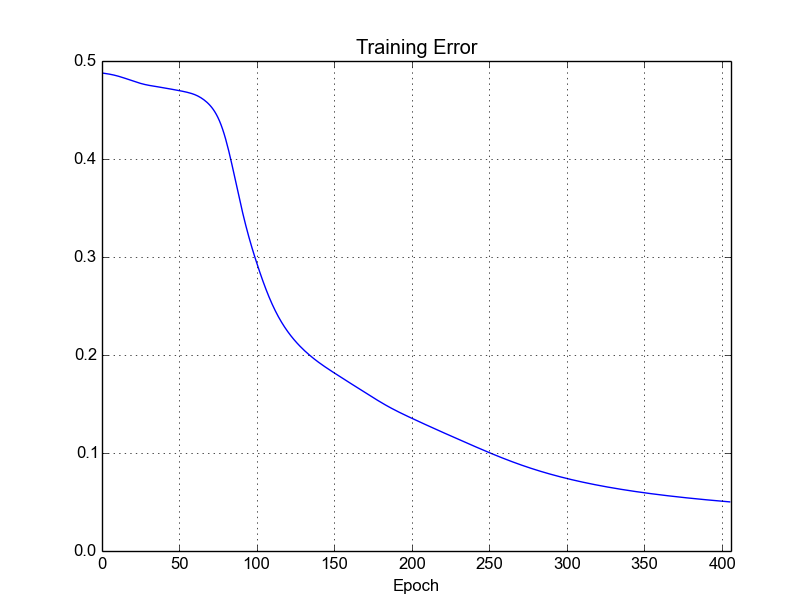
\includegraphics[width=\linewidth]{fig/trainingerror_lr0,0075_eps0,05_regparam0,00_beta5_batch1.png}
	\end{subfigure}
	\begin{subfigure}[b]{0.5\textwidth}
		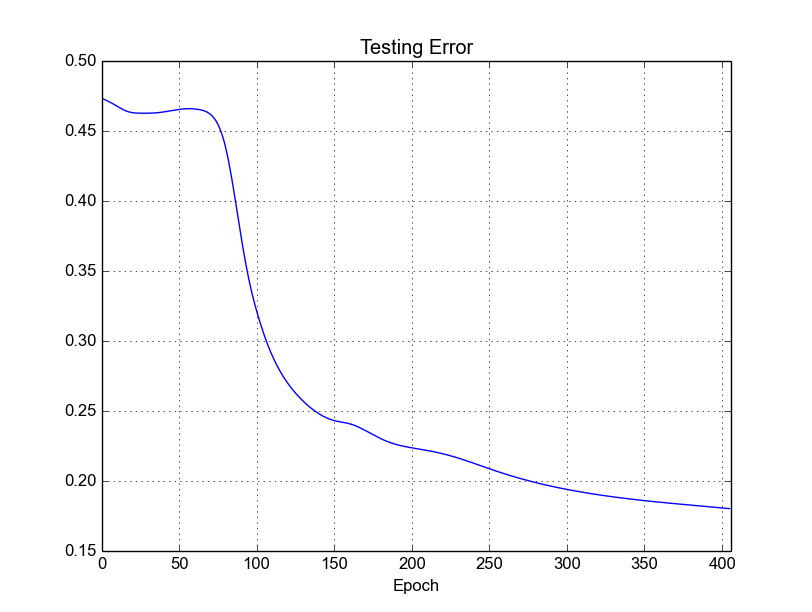
\includegraphics[width=\linewidth]{fig/valerror_lr0,0075_eps0,05_regparam0,00_beta5_batch1.png}
	\end{subfigure}

	\caption{\textbf{learning rate: 0.0075}}
\end{figure}


\begin{figure}[h]	
	\begin{subfigure}[b]{0.5\textwidth}
		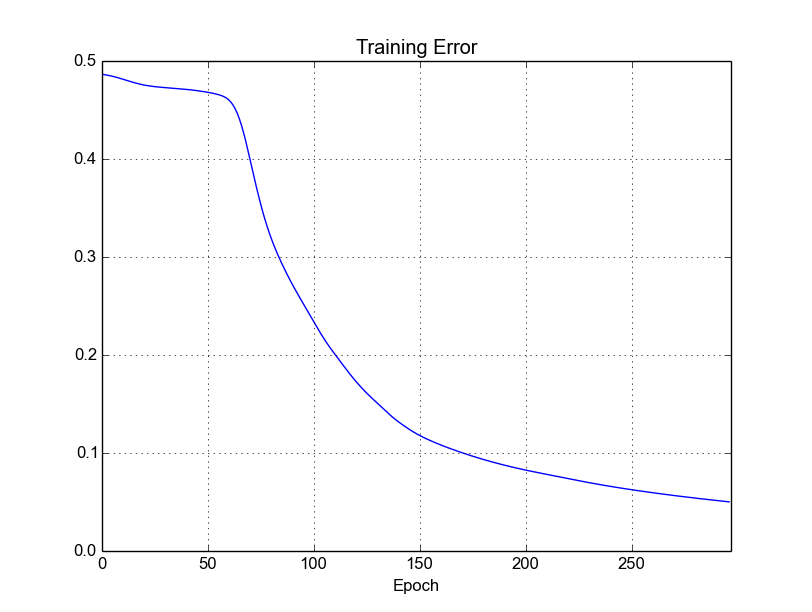
\includegraphics[width=\linewidth]{fig/trainingerror_lr0,01_eps0,05_regparam0,00_beta5_batch1.png}
	\end{subfigure}
	\begin{subfigure}[b]{0.5\textwidth}
		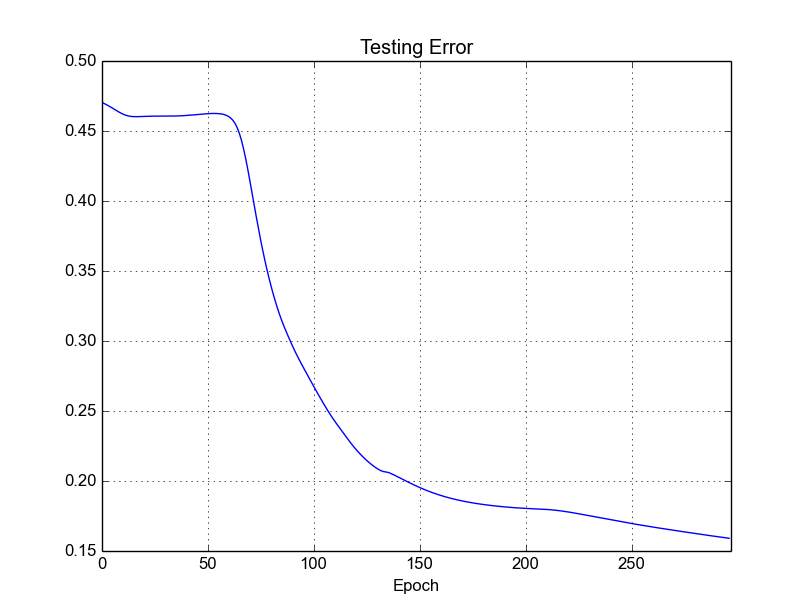
\includegraphics[width=\linewidth]{fig/valerror_lr0,01_eps0,05_regparam0,00_beta5_batch1.png}
	\end{subfigure}

	\caption{\textbf{learning rate: 0.01}}
\end{figure}

En estos gráficos se puede ver que el error fue menor a epsilon = 0,05.
 En el primero de ellos el coeficiente de aprendizaje utilizado es 
 0.0075 y en el segundo 0.01. Se observa que coeficiente de aprendizaje
  más pequeño el error sube. Por otro lado, se puede ver que cuanto 
  más chico paso más épocas fueron necesarias para minimizar el error. 
Por lo que elegimos 0.01 como mejor learning rate.

\newpage

\begin{figure}[h]	
	\begin{subfigure}[b]{0.5\textwidth}
		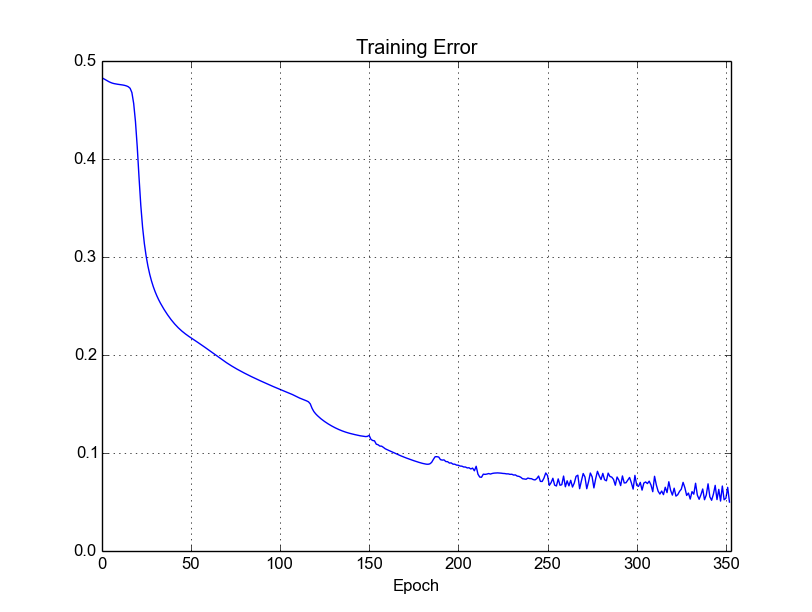
\includegraphics[width=\linewidth]{fig/trainingerror_lr0,025_eps0,05_regparam0,00_beta5_batch1.png}
	\end{subfigure}
	\begin{subfigure}[b]{0.5\textwidth}
		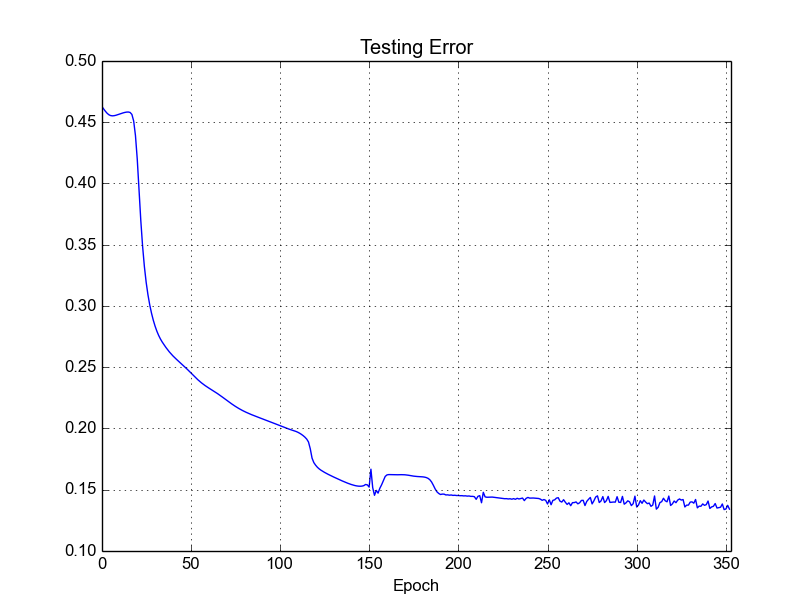
\includegraphics[width=\linewidth]{fig/valerror_lr0,025_eps0,05_regparam0,00_beta5_batch1.png}
	\end{subfigure}

	\caption{\textbf{learning rate: 0.025}}
\end{figure}



\begin{figure}[h]	
	\begin{subfigure}[b]{0.5\textwidth}
		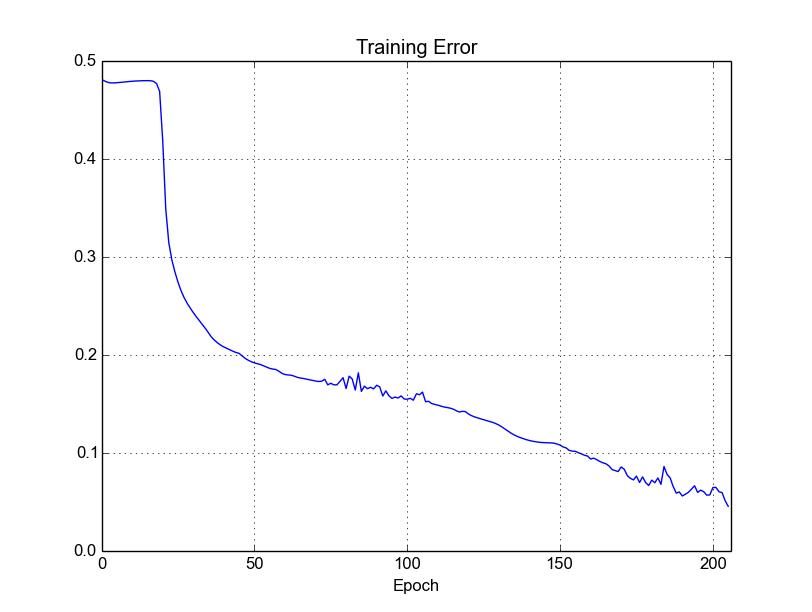
\includegraphics[width=\linewidth]{fig/trainingerror_lr0,05_eps0,05_regparam0,00_beta5_batch1.png}
	\end{subfigure}
	\begin{subfigure}[b]{0.5\textwidth}
		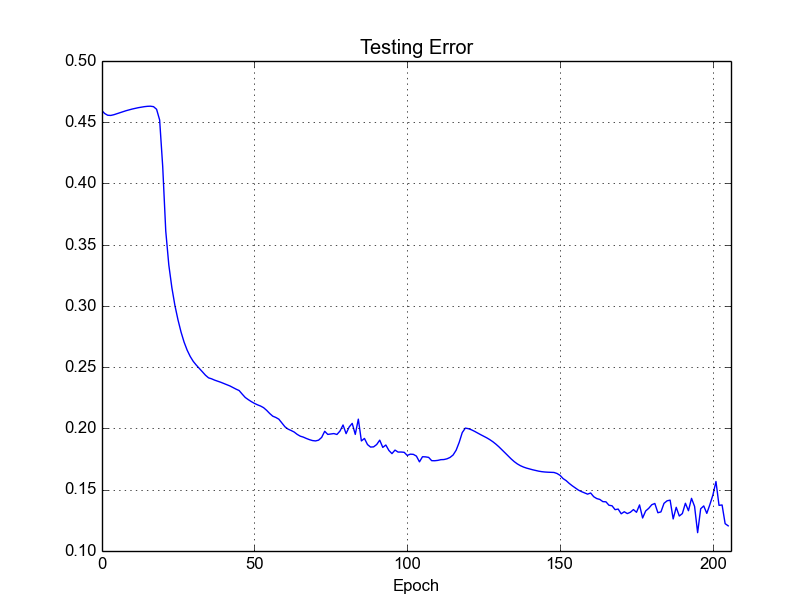
\includegraphics[width=\linewidth]{fig/valerror_lr0,05_eps0,05_regparam0,00_beta5_batch1.png}
	\end{subfigure}

	\caption{\textbf{learning rate: 0.05}}
\end{figure}



Estos dos gráficos muestran que al ser el coeficiente de aprendizaje es
 muy grande y se han encontrado mínimos locales por lo que el error empezó
  a oscilar. En estos casos, el error también fue menor a epsilon = 0.05 
  pero fueron necesarias mayor cantidad de épocas para hacerlo. Estos 
  learning rate no son óptimos para este modelo por lo que no son 
  los elegidos.

\newpage

\subsection{Modo de Uso}

Aclaración: por falta de tiempo no hicimos el preprocesamiento automático de los atributos del archivo de entrada del ej1 que figuran como letras y los modificamos a mano para reemplazar B=0 M=1.

Para entrenar la red:

Ejemplo: 

\noindent\texttt{\scriptsize{python trainnet1.py -m TP1/models/ej1.lmodel -o ./salida.params -t 900 -e 0.05 -l 0.005 -b 1 -x TP1/ds/tp1\_ej1\_training.csv}}

Explicación:

\begin{tabular}{ l l }
-m & Ruta al archivo de modelo (lmodel) \\
-o & Ruta del archivo de salida con los pesos\\
-t & Epochs\\
-e & Epsilon\\
-l & Learning rate\\
-b & Size minibatch (default 1)\\
-x & Archivo de samples\\
\end{tabular}

\begin{tabular}{ c l }
-m M & Ruta al archivo de modelo (lmodel)\\
-p  O & Ruta del archivo de entrada con los pesos\\
-x  X & Archivo de features\\
\end{tabular}

Para predecir (el formato tiene que ser el mismo que el de entrenamiento):

\begin{tabular}{ l l }
-m & Ruta al archivo de modelo (lmodel)\\
-p & Ruta del archivo de entrada con los pesos\\
-x & Archivo de features\\
\end{tabular}
